% !TeX root = ./00.main.tex
\chapter{Fundamentos Científicos e Tecnológicos}\label{cha:fundamentos}

% cap 2: fundamentos científicos e tecnológicos
%     (pegue apenas os mais citados, siga a Elaine)
%     2.1. Computação em Nuvem, Fog e Edge
%     2.2. Plataformas de processamento distribuído
%         - arq lambda, kappa, (vide guilherme)
%         - MapReduce, Hadoop, Spark, Storm
%     2.3. Apache Flink
%     2.4. Mineração de Dados
%     2.5. Mineração de Stream
%         - quem são, o que consomem
%         (BigFlow apud \cite{Gaber2005}) Mining data streams: A Review.
%     2.6. Novelty Detection
%     2.7. O algoritmo Minas

% \notahermes{Seria bom incluir algum texto aqui, pelo menos um paragrafo dizendo do que
% trata este capitulo }

\begin{resumocap}
  Este Capítulo aborda conceitos que embasam esse trabalho,
  conceitos teóricos de
  ambientes e arquiteturas de computação distribuída e detecção de novidade
  e conceitos técnicos, como plataformas de processamento distribuído de fluxo
  de dados e o algoritmo MINAS.
\end{resumocap}

\section{Ambientes de Computação Distribuída}

\newcommand{\cloud}{\emph{cloud computing}\xspace}

% \notahermes{Falta algum texto introdutorio aqui, fazendo a
% ``cola'' entre as 3 plataformas.  \\  Se você não conseguir fazer essa ``cola''
% (isto é, pensar em um titulo de seção melhor e colocar o texto, pode
% simplesmente remover a seção 2.1 e promover as 3 subseções (computação em nuvem,
% borda e Fog) para o nível de seção. }

Esta \Section relaciona três ambientes de computação distribuída habitualmente
utilizados para o processamento de dados massivos relacionados a redes de
dispositivos \iot, entre outras aplicações.
% Iniciando com o ambiente \hlhl{mais tradicional},
\notafa{rever a frase} \hlfa{A computação em nuvem (\cloud) é}
aplicada a vários problemas e neste trabalho seu papel em sistemas \iot é
fornecer \notahl{?}\hlhl{vastos recursos e garantias e em que dispositivos}
\hlhl{enviam todos dados} \hlhl{relevantes ao sistema}.
O segundo e terceiro ambiente são computação de borda (\emph{edge computing})
e a computação em névoa (\emph{fog computing}), que utiliza os recursos
computacionais distribuídos presentes em nós localizados entre os dispositivos
de borda e a nuvem, com diversas 
intenções, desde privacidade até redução de latência.
% \notafa{por favor, use um corretor ortográfico. Intenção}

% Para descrever os modelos de computação em nuvem, borda e névoa, é necessário
% abordar o conceito de distância e densidade em redes. Distância pode ser definida 
% como o número de saltos (\emph{hops}), latência, distância geográfica ou combinação destas.
% Densidade é extraída da distância, projetando a mesma num hiper-espaço de maneira que os
% nós com menor distância entre si fiquem mais próximos. Então quando existe um
% grande número de nós numa mesma região diz-se que ela é densa, quando há poucos
% nós em uma região, esparsa. Acredita-se que data centers, backbones e nuvens publicas
% formem uma concentração de nós e quanto mais próximo do usuários finais (folhas)
% mais esparso é esse hiper-espaço.

% Definir internet e rede (borda, centro, etc)
% Classificando a internet por sua densidade podemos dizer que ao centro estão
% os \emph{data centers} e nuvens públicas em seguida o núcleo interconectando redes diversas,
% redes locais e a Borda composta pelos nós folha dentro de uma rede local.

% O modelo de Computação em Nuvem (\emph{Cloud Computing})
% permite alocar recursos como redes, servidores, armazenamento, aplicações    e serviços
% de maneira conveniente e seu provisionamento ágil concede elasticidade para atender
% demandas variáveis com custo mínimo \cite{NIST2011}.

% Definição de Cloud Computing

\subsection{Computação em Nuvem}

A computação em nuvem (\cloud), ou simplesmente nuvem
(\emph{cloud}), habilita o acesso através da rede a um grupo compartilhado de
recursos de computação configuráveis (servidores, redes, aplicativo,
\notafa{frase grande, falta de pontuação. O leitor se perde!}
armazenamento, serviços, etc.), que podem ser provisionados ou liberados sob
demanda rapidamente com o mínimo esforço de gerenciamento ou interação com o
\hlhl{provedor de serviços} \cite{NIST2011}.
\notahl{o texto pode ficar mais claro se você evitar inversões na estrutura
da frase e usar parágrafos curtos.}
As principais características do ambiente \cloud, segundo \citeonline{NIST2011}
são:
% \notafa{referencia}

% Alternativamente, a Computação na Borda (\emph{Edge Computing}) destaca-se no
% processamento em tempo real de dados originários da própria borda além de atender
% preocupações de segurança e privacidade \cite{Shi2016}.

\begin{itemize}
    
    \item \textbf{Serviço sob Demanda:} o cliente pode provisionar ou liberar
    capacidades de computação (ex: tempo de processamento e armazenamento) conforme o
    necessário, sem requerer interação com o provedor de serviço;
    
    \item \textbf{Amplo acesso à rede:} o acesso aos recursos de computação e
    capacidades ocorre pela rede através de mecanismos padrões que permitem o
    acesso por plataformas heterogêneas (celulares, computadores, tablets, etc.)
      
    \item \textbf{Agrupamento de recursos:} para servir múltiplos clientes, os
    recursos de computação são agrupados usando o modelo \emph{multi-tenancy}
    com recursos físicos e virtuais diferentes dinamicamente atribuídos e
    reatribuídos de acordo com a demandas do clientes;
    
    \item \textbf{Elasticidade:} as capacidades de computação são rapidamente
    provisionadas ou liberadas, em alguns casos automaticamente, para escalar
    conforme a demanda;
    
    \item \textbf{Serviço mensurado:} os recursos de computação são monitorados,
    controlados e reportados para o provedor de serviços e para o cliente
    fornecendo transparência sobre as capacidades que foram consumidas.

\end{itemize}

Segundo, \citeonline{NIST2011}, a implantação da Computação em Nuvem pode
ocorrer através dos seguintes modelos:

\begin{itemize}
    
    \item \textbf{Nuvem privada:} a infraestrutura da nuvem é provisionada e
    dedicada para um único cliente ou organização. Nesse modelo, o cliente
    gerencia e controla a infraestrutura, ou pode delegar essas tarefas a uma
    outra empresa. A infraestrutura pode estar dentro ou fora das instalações
    da organização proprietária;

    \item \textbf{Nuvem comunitária:} a infraestrutura de nuvem é fornecida para
    um grupo exclusivo de clientes que compartilham um mesmo interesse
    (requerimentos de segurança, desempenho, políticas, etc.). Esse tipo de
    nuvem pode ser gerenciado pelo próprio grupo, ou por outra organização,
    podendo estar dentro ou fora das instalações das empresas proprietárias;

    \item \textbf{Nuvem pública:} É gerenciada e operada por um provedor de nuvem
    e a infraestrutura é provisionada e oferecida para uso público.
    
    \item \textbf{Nuvem híbrida:} a infraestrutura desse tipo de nuvem é uma
    composição de dois ou mais modelos de implantação de \emph{cloud} (privada,
    pública e comunitária) que formam uma entidade única e são unidos por
    tecnologias padronizadas que habilitam a portabilidade de dados e
    aplicações.

\end{itemize}

% Definição de Computação de Borda 
\subsection{Computação de Borda}

\notafa{repare que cada uma das seções referencia um único autor. Seria interessante ter várias referências}
\hlfa{A computação de borda} (\emph{edge computing}) refere-se às
tecnologias que permitem que a computação seja executada na borda da rede.
Define-se borda ou \emph{edge} como qualquer recurso de computação e de rede ao
longo do caminho entre as fontes de dados e os data centers da nuvem
\cite{Shi2016}. Na borda, é possível fazer armazenamento, processamento e
descarregamento de dados, assim como distribuir as requisições e entregar os
serviços das nuvens aos usuários. \citeonline{Shi2016} ressalta que essas
capacidades (dentre outras) dos nós da borda (\emph{edge nodes}) possibilitam que a
computação de borda reduza a latência na resposta da nuvem, pré-processando os
dados nos nós da borda, aproveitando melhor a banda e a transmissão de dados, e
também consumindo menos recursos de computação na nuvem. Além disso, o autor
ainda acrescenta que a computação de borda pode aumentar a privacidade dos
dados, uma vez que eles podem ser processados no próprio dispositivo final.

A computação de borda tenta trazer a computação mais próxima das fontes de
dados.
% , como mostra a Figura \ref{edge-computing}
Como é observado na figura, os
componentes desse tipo de computação podem ser tanto produtores como
consumidores, não só requisitando serviços e conteúdo da nuvem, mas também
realizando tarefas da nuvem.
Algumas aplicações da computação de borda incluem: análise de vídeo;
em sistemas críticos para redução de latência;
descarregar a nuvem de parte da computação;
privacidade dos dados produzidos, mantendo-os fora de ambientes públicos;
redução das cargas de dados na rede e
processamento distribuído de sensoriamento massivo em cidades inteligentes \cite{Shi2016}.

\notake{deixar figura em portugês}
% \begin{figure}[hbt]
% \centering
% 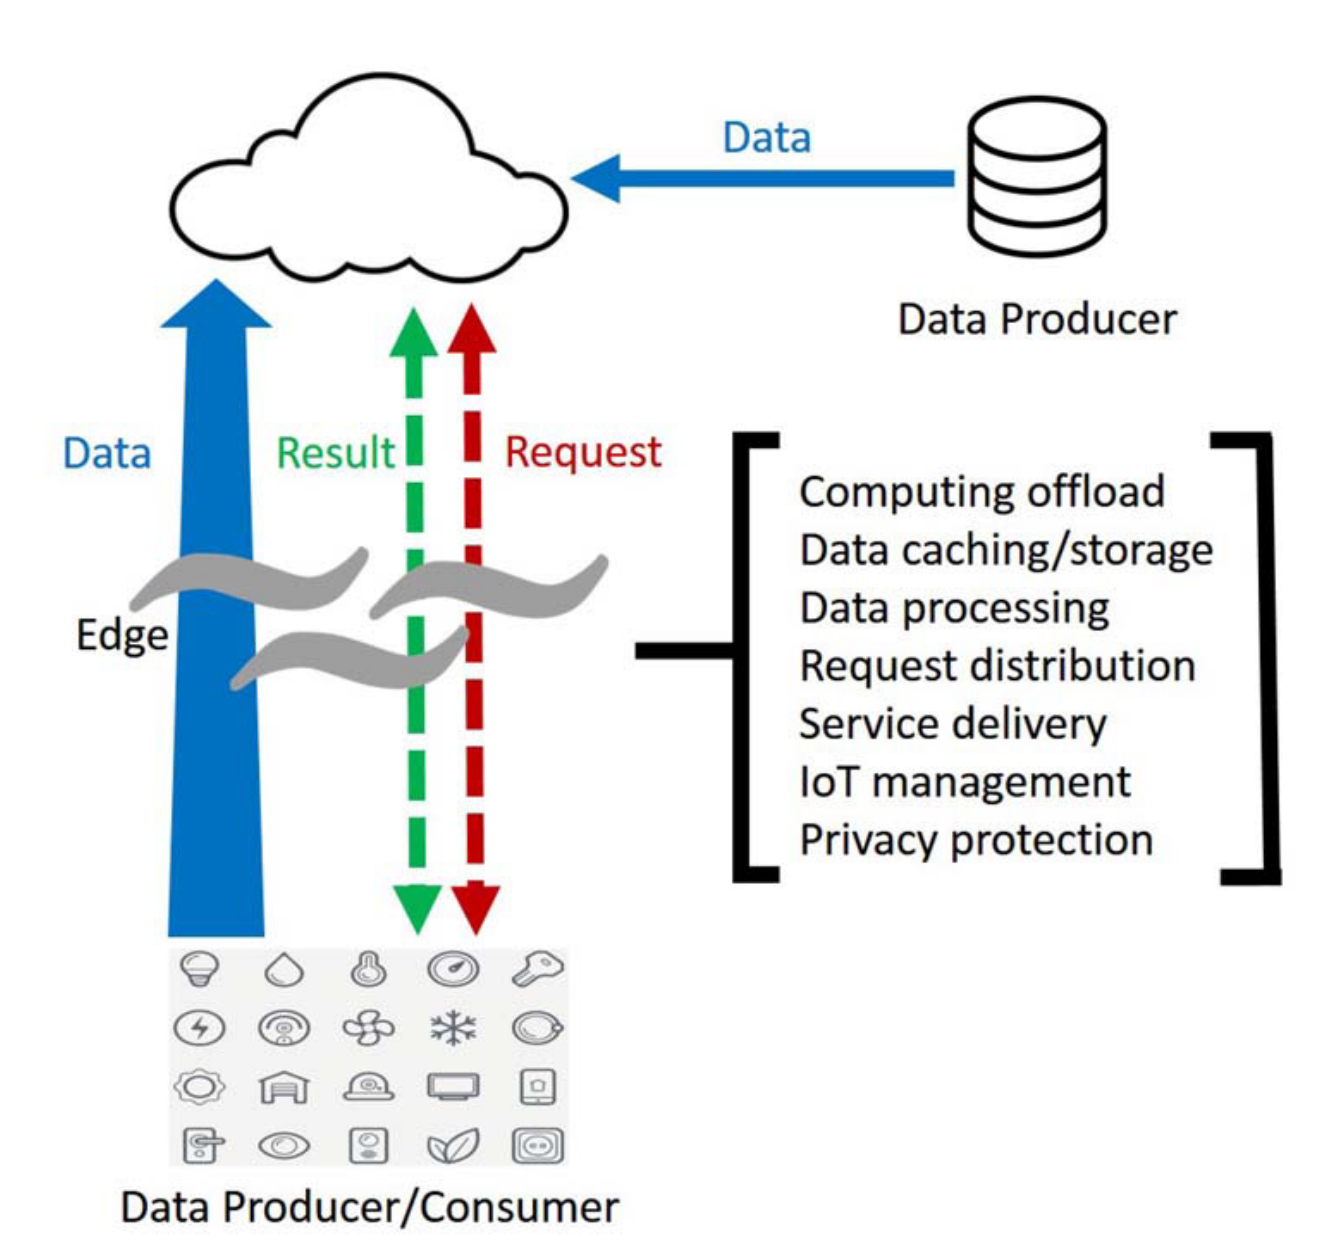
\includegraphics[width=0.6\textwidth]{figuras/edge-computing.png}
% \caption{Paradigma de \emph{Edge Computing} \cite{Shi2016}.}
% \label{edge-computing}
% \end{figure}

\subsection{Computação em Névoa}

\citeonline{Dastjerdi2016} e \citeonline{IEEECommunicationsSociety2018}
mencionam que a enorme massa de dados gerados por ambientes IoT pode ser
processada em nuvem, entretanto \hlhl{a latência} produzida pela transferência desses
dados para a nuvem e o retorno do resultado pode não ser toleradas por sistemas
críticos que sejam sensíveis a latência (monitoramento de saúde e resposta a
emergências).
\citeonline{IEEECommunicationsSociety2018} ainda acrescenta que enviar tantos
dados à nuvem
para processamento e armazenamento pode ser ineficiente e não escalável, devido à
saturação de dados na rede.
O ambiente \emph{edge computing} foi proposto para trazer o
processamento e armazenamento para os dispositivos de borda tentando solucionar
esses problemas.
Porém, dispositivos de borda comumente não podem lidar com várias
aplicações IoT competindo pelos seus recursos limitados, o que poderia causar a
contenção dos recursos e o aumento na latência do processamento
\cite{Dastjerdi2016}. Portanto, para solucionar estas questões de latência e
capacidade limitada dos dispositivos de borda, a computação em névoa foi proposta.

A computação em névoa (\emph{fog computing}) é um paradigma que distribui
as capacidades de computação, armazenamento e rede entre os nós próximos
\hlhl{das fontes dados}
\notahl{nós finais não são as fontes?}
e dos \hlhl{dispositivos finais}, mas não necessariamente localizados na borda,
dando a esses nós características de uma nuvem
\cite{Bonomi2012,Dastjerdi2016,IEEECommunicationsSociety2018}.
Esse tipo de computação evita a sobrecarga dos dispositivos de borda.
\citeonline{Bonomi2012} e
\citeonline{Dastjerdi2016} consideram computação em névoa como complementar da
computação em borda, podendo a computação em névoa aproveitar os recursos da
nuvem e da borda.
\citeonline{IEEECommunicationsSociety2018} considera que a
principal diferença entre esses dois tipos de computação está no número de
camadas.
Enquanto \emph{edge computing} tem
\notahl{o que são ``camadas''?}\hlhl{camadas menores}, pois atua só nos
dispositivos de borda, \emph{fog computing} tem mais camadas e um modelo
hierárquico, pois não atua só na camada de borda.

Segundo \citeonline{Bonomi2012} e \citeonline{Dastjerdi2016}, as principais
características da computação em névoa são:

\begin{itemize}

    \item \textbf{Mobilidade:} é essencial que as aplicações \emph{fog} sejam
    capazes de se comunicar com dispositivos móveis, por exemplo, utilizando
    protocolos que considerem a mobilidade dos nós;

    \item \textbf{Heterogeneidade:} os nós nesse tipo de paradigma possuem
    configurações e formatos diferentes e podem estar implantados em ambientes
    distintos;

    \item \textbf{Baixa Latência:} \hlhl{computação em névoa} foi proposta para
    atender aplicações que requeiram baixa latência (monitoramento de saúde,
    jogos, realidade aumentada, etc.);

    \item \textbf{Distribuição geográfica:} computação em névoa pode possuir
    milhares de sensores e dispositivos distribuídos geograficamente, com
    consciência de suas localizações (\emph{location awareness});

    \item \textbf{Alto número de nós:} seguindo os ambientes IoT, a computação
    em névoa pode ser composta por milhares de nós;

    \item \textbf{Interoperabilidade e federação:} os componentes da computação
    em névoa devem ser capazes de interoperar, e o serviços devem ser federados
    \hlhl{ao longo de diferentes domínios};

    \item \textbf{Uso de fluxo de dados e aplicações em tempo real:} a
    computação em névoa pode envolver aplicações que processam em lote, mas na
    maior parte das vezes envolve aplicações com requisito de processamento em
    tempo real, e para isso fazem o uso de fluxo de dados. Por exemplo, os
    sensores de um rede IoT escrevem a informação no fluxo de dados, a
    informação é processada, ações são inferidas e traduzidos em
    ações nos componentes atuadores.

\end{itemize}

Algumas aplicações para computação em névoa são:
cidades inteligentes e
semáforos inteligentes que enviam sinais de alerta aos veículos e coordenam os
sinais verdes com outros semáforos através de sensores (veículos, pedestres,
ciclistas);
na área de saúde, para monitorar e prever situações de pacientes que
estão conectados a sensores;
em prédios inteligentes, que são dotados de sensores
de umidade, temperatura, qualidade do ar, ocupação, sendo que a partir das
informações deles, é possível alertar os ocupantes do prédio em algum caso de
emergência.

\section{Mineração de Dados e Fluxo de Dados}

% Faria nem Silva definem ou citam data mining
% A data stream (DS) is a sequence of examples that arrive continuously. They are
% continuous, unbounded, flow at high speed and have a data distribution that
% may change over time \cite{Silva2013}. In DS scenarios, new concepts may
% appear and known concepts may disappear or evolve. \cite{Faria2016nd}

A Mineração de Dados é o processo de descoberta de padrões em conjuntos de dados
utilizando métodos derivados de aprendizagem de máquina, estatística e banco de
dados \cite{Gaber2005}.
\notafa{eu não acho que Big Data é uma caso de mineração}
\hlfa{Um caso de mineração} de dados é o \emph{Big Data}, enque o
conjunto de dados comumente não pode ser processado em tempo viável, devido a limitações
como memória ou armazenamento principal.

% Data stream mining is concerned with the extraction of knowledge from large
% amounts of continuously generated data in a non-stationary environment. Novelty
% detection (ND), the ability to identify new or unknown situations not
% experienced before, is an important task for learning systems, especially when
% data are acquired incrementally (Perner 2008). In data streams (DSs), where new
% concept can appear, disappear or evolve over time, this is an important issue to
% be addressed. ND in DSs makes it possible to recognize the novel concepts, which
% may indicate the appearance of a new concept, a change in known concepts or the
% presence of noise (Gama 2010).
% 
% Perner P (2008) Concepts for novelty detection and handling based on a case-based
% reasoning process scheme. Eng Appl Artif Intell 22:86–91
% 
% Gama J (2010) Knowledge discovery from data streams, vol 1, 1st edn. CRC press chapman hall, Atlanta

% dados massivamente e continuamente gerados e não persistentes. Fp

% \cite{Gaber2005} Cited by 1174
% Data mining is that interdisciplinary field of study that can extract models
% and patterns from large amounts of information stored in data repositories
% [30, 31, 34].
% 
% Recently, the data generation rates in some data sources become faster than ever
% before. This rapid generation of continuous streams of information has
% challenged our storage, computation and communication capabilities in computing
% systems. Systems, models and techniques have been proposed and developed over
% the past few years to address these challenges [5, 44]

Além da dimensão de armazenamento, outra dimensão que afeta a maneira como dados
são modelados e manipulados é o tempo.
\notafa{rever a definição. Você referencia o Gaber (autor do any novel), mas eu não
encontrei essa definição lá. Use definições classicas como as do João, do
Aggarwal.}
\hlfa{Um Fluxo de Dados} (\emph{Data Stream}) é
uma sequência de registros
% produzidos a uma taxa muito alta,
associados ao tempo
real, ilimitados, que excede recursos de armazenamento \cite{Gaber2005}.
\notafa{o que são modelo de mineração?
Um modelo é produzido a partir de um algoritmo de mineração}
\hlfa{Modelos de mineração} de fluxo de dados atendem a esses desafios utilizando
restrições \hlhl{como apenas uma leitura do conjunto de dados} e baixo tempo de
processamento na construção de seus algoritmos \cite{Gama2007, Gaber2005}.

% \notahermes{Não faz sentido considerar como fluxo somente se a taxa for muito alta.
% Precisa rever isto.}

% \notahermes{O que é complexidade menor que linear em fluxos? }

% \nota{falta abordar processamento paralelo e distribuído}

As características de fluxos de dados e mineração de dados e os requisitos de
seu processamento regularmente superam as capacidades computacionais de um único
nó computacional convencional, de forma que a distribuição dos requisitos em
múltiplos nós computacionais em um sistema distribuído pode ser necessária
\cite{Gaber2005}.

Computação distribuída é a área da ciência da computação que estuda sistemas
em que os componentes são localizados em diferentes computadores (nós), que
comunicam-se apenas por troca de mensagens e, para que o objetivo do sistema
seja atingido, a cooperação entre os nós é necessária.
Outras propriedades de um sistema distribuído são a concorrência entre os nós e
possibilidade de
falhas em partes independentes \cite{TanenbaumSteen2018}.

% - quem são, o que consomem
% (\citeonline{Viegas2019} \emph{apud} \citeonline{Gaber2005}) Mining data streams: A Review.
% {Gaber2005} apud [47] {Park2002distributed}
% [47] B. Park and H. Kargupta. Distributed Data Mining: Algorithms, Systems, and
% Applications. To be published in the Data Mining Handbook. Editor: Nong Ye.
% 2002.]

% A data stream is a sequence of unbounded, real-time data records that are
% characterized by the very high data rate, which stresses our computational
% resources, and can be read only once by processing applications [13,8,1,9]
 
% [1] B. Babcock, S. Babu, M. Datar, R. Motwani, J. Widom, Models and issues in
% data stream systems. In: Proceedings of Principles of Database Systems
% (PODS’02), pp. 1–16, 2002. \cite{Babcock2002}

% [2] G. Boone, Reality mining: browsing reality with sensor networks.
% In: Sensors Online, vol. 21, 2004.

% [3] V. Cantoni, L. Lombardi, P. Lombardi, Challenges for data mining in
% distributed sensor networks. ICPR (1) 1000–1007, 2006

% [8] M.M. Gaber, A. Zaslavsky, S. Krishnaswamy, Mining data streams: a review.
% ACMSIGMOD Record, 34(2):18–26, 2005.
% 
% [9] M. Garofalakis, J. Gehrke, R. Rastogi, Querying and mining data streams:
% you only get one look a tutorial. In: Proceedings of the 2002 ACM SIGMOD
% International Conference on Management of Data, June 03–06, Madison, Wisconsin,
% 2002.
% 
% [13] S. Muthukrishnan, Data streams: algorithms and applications. In:
% Proceedings of the Four- teenth Annual ACM-SIAM Symposium on Discrete
% Algorithms, 2003.

% Mineração de Fluxo de Dados é análogo à mineração de
% dados e \emph{big data} com a restrição temporal onde um registro é unicamente 
% associado um tempo, dessa forma além de não ser possível manipular o conjunto
% de dados em memória, não é possível recuperar dados fora do intervalo de tempo associado
% a eles.

% ----- wikipedia ------
% 
% Data mining is the process of discovering patterns in large data sets involving
% methods at the intersection of machine learning, statistics, and database
% systems.[1] Data mining is an interdisciplinary subfield of computer science and
% statistics with an overall goal to extract information (with intelligent
% methods) from a data set and transform the information into a comprehensible
% structure for further use.[1][2][3][4] Data mining is the analysis step of the
% "knowledge discovery in databases" process or KDD.[5] Aside from the raw
% analysis step, it also involves database and data management aspects, data
% pre-processing, model and inference considerations, interestingness metrics,
% complexity considerations, post-processing of discovered structures,
% visualization, and online updating.[1]
% 
% [1] "Data Mining Curriculum". ACM SIGKDD. 2006-04-30. Retrieved 2014-01-27.
% [2] Clifton, Christopher (2010). "Encyclopædia Britannica: Definition of Data Mining". Retrieved 2010-12-09.
% [3] Hastie, Trevor; Tibshirani, Robert; Friedman, Jerome (2009).
% "The Elements of Statistical Learning: Data Mining, Inference, and Prediction".
% Archived from the original on 2009-11-10. Retrieved 2012-08-07.
% [4] Han, Kamber, Pei, Jaiwei, Micheline, Jian (June 9, 2011).
% Data Mining: Concepts and Techniques (3rd ed.). Morgan Kaufmann. ISBN 978-0-12-381479-1.
% [5] Fayyad, Usama; Piatetsky-Shapiro, Gregory; Smyth, Padhraic (1996).
% "From Data Mining to Knowledge Discovery in Databases" (PDF). Retrieved 17 December 2008.

\notafa{ aqui o parágrafo ficou perdido. Ao fim de seção de mineração você vai
falar de computação distribuída}

\section{Arquiteturas e Plataformas de Processamento de Fluxos}

% - arq lambda, kappa, (vide guilherme)

% Existem diversas maneiras de organizar o caminho das informações em um
% aplicativo de processamento de fluxo de dados. Algumas propostas sao amplamente
% conhecidas como as arquiteturas Lambda (MARZ; WARREN, 2015) e Kappa (KREPS,
% 2014), as quais s˜ao genéricas e focadas no processamento de fluxo.

% A arquitetura Lambda (MARZ; WARREN, 2015) mescla o processamento do fluxos de
% dados com o processamento em lotes. O objetivo dessa mistura é obter, ao mesmo
% tempo, a capacidade de fazer análises em tempo real, e, ao mesmo tempo,
% fazê-las com maior qualidade. Seu processamento é dividido em duas camadas,
% uma camada de processamento online que fornece resultados aproximados com baixa
% latência e uma camada de processamento offline que usa os dados históricos
% disponíveis e fornece resultados mais precisos, embora com maior sobrecarga e
% latência. Além das duas camadas de processamento, a Arquitetura Lambda possui
% uma camada de serviço, que combina dados de ambas as camadas de processamento e
% apresenta ao usuário.

% A arquitetura Kappa, por outro lado, possui apenas as camadas de processamento e
% serviço de fluxo. Seu objetivo é o processamento em tempo real, portanto
% possui a menor quantidade possível de sobrecarga e latência. Sendo assim, é
% natural que esta seja uma arquitetura muito simples e que possua apenas os
% módulos essenciais para um sistema de processamento de fluxo. A arquitetura
% Kappa possui apenas um módulo de processamento on-line que opera através do
% fluxo de dados e fornece informações.

% MARZ, N.; WARREN, J. Big Data: Principles and Best Practices of Scalable
% Realtime Data Systems. 1st. ed. Greenwich, CT, USA: Manning Publications Co.,
% 2015. ISBN 1617290343, 9781617290343. \cite{marz2015big}

% KREPS, J. Questioning the Lambda Architecture. 2014. Disponível em:
% https://www.oreilly.com/ideas/questioning-the-lambda-architecture

% \notahermes{Os conceitos ficaram um tanto misturados nesta seção.
% Acho que ficaria 
% melhor se dividisse em 2 ou 3 seções, por exemplo: uma seção sobre processamento
% em batch ou {\it offline} como Mapreduce/Hadoop, ou o Spark originalmente;
% uma segunda seção poderia falar somente de plataformas de processamento de fluxos;
% terceira poderia falar sobre as arquiteturas (lambda, kappa) que combinam de
% certa forma as plataformas offline e de fluxos. Acho que kafka poderia aparecer
% dentro dessa terceira seção.}

Tradicionalmente, \notahl{quais? de que tipo?}\hlhl{aplicações} foram construídas com um sistema gerenciador de
banco de dados (SGBD) relacional ou não-relacional associado. Essa arquitetura,
nomeada de arquitetura totalmente incremental por \citeonline{marz2015big},
foi evoluída e simplificada iterativamente durante décadas de uso, porém ela não
é adequada para sistemas em 
\notafa{o que é tempo real}
\hlfa{tempo real}, como os sistema de fluxo de dados.
O volume e a velocidade de dados em um \emph{Data Stream} leva à necessidade de
distribuir o processamento, acrescentando poder computacional a cada nó
adicionado.
Porém, desafios como comunicação eficiente e sincronização de estado
entre os nós, assim como tolerância a falhas, aumentam a complexidade de
construção de um sistema distribuído em relação a um sistema tradicional.

% \notahermes{Eu nem citaria SGBD, isso foi novidade há uns 30 ou 40 anos. Mapreduce já
% tem praticamente 20 anos ... }
% \nota{citei somente para ter uma base introdutória, seguindo o livro \cite{marz2015big}}

\newcommand{\lambdaa}{\xspace\emph{Lambda}\xspace}
\newcommand{\kappaa}{\xspace\emph{Kappa}\xspace}

Para mitigar problemas associados à construção de sistemas \emph{Big Data}
e \emph{Data Streams},
arquiteturas de processamento de fluxo
de dados distribuído foram propostas, como a arquitetura \lambdaa
\cite{marz2015big} e \kappaa \cite{Kreps2014}, além
de
diversas plataformas, tanto de \emph{Big Data} com características de tempo real,
como especializadas em fluxo de dados.

% \notahermes{Tem referências para Lambda e Kappa? }

\subsection{Arquitetura \lambdaa \notahl{do quê?}}

A arquitetura de processamento distribuído de fluxos de grande volume de dados
\lambdaa divide o processamento em três camadas:
\notahl{isso é camada?}\hlhl{lotes, serviço e velocidade} \cite{marz2015big}.
A camada de lotes atua sobre o 
\notafa{o que é conjunto mestre?}
\hlfa{conjunto} \hlhl{mestre}
 em modo de leitura
sequencial, armazenando-o em sistema de arquivos distribuído e pré-processando
várias visões sobre esse conjunto mestre.
Essas visões (armazenadas num SGBD
tradicional) são consumidas pela camada de serviço, que portanto tem acesso
regular (leitura aleatória) dos dados.
No entanto, as garantias oferecidas pela camada de
lotes (escalabilidade, consistência, tolerância a falhas) não atendem os requisitos
de latência em um sistema em tempo real, para isso a camada de velocidade
complementa os dados das visões com dados diretamente do conjunto mestre em
tempo real diretamente para a camada de serviço \cite{marz2015big}.

% A Figura \ref{fig:lambda} ilustra uma implementação da arquitetura \lambdaa
% onde \emph{Apache Kafka}, \emph{Apache Storm}, \emph{Apache Hadoop}
% implementam o conjunto mestre, camada de velocidade e camada de lotes
% respectivamente.

% \notafa{aqui vale o mesmo questionamento da figura 2.1}
% \begin{figure}[ht]
% \centering
% 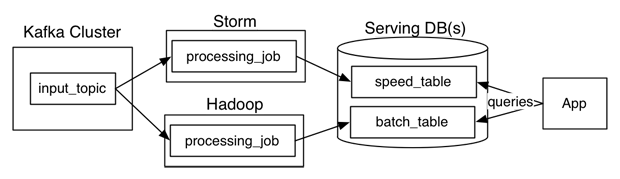
\includegraphics[width=0.6\textwidth]{figuras/lambda.png}
% \caption{Arquitetura \lambdaa com detalhes práticos \cite{Kreps2014}.}
% \label{fig:lambda}
% \end{figure}

\subsection{Arquitetura \kappaa}

Em contraposição à arquitetura \lambdaa, observações práticas de 
\citeonline{Kreps2014} mostram que o sistema de fila de mensagens
(no exemplo \emph{Apache Kafka}) já traz as garantias de
escalabilidade, consistência, tolerância a falhas, replicação e armazenamento de longo prazo.
Com isso, \citeonline{Kreps2014} propõe que as camadas de lotes e velocidade sejam
unificadas em uma camada de processamento de fluxo, cujos resultados sejam entregues
continuamente para a camada de serviço através de um SGBD, definindo assim a arquitetura \kappaa.
Essa proposta simplifica a aplicação de três implementações para duas, eliminando a
repetição de tarefas executadas pelas camadas de lotes e velocidade que
produziam o mesmo resultado.

% A arquitetura \kappaa limita-se ao processamento de \emph{Stream} apenas
% \emph{on-line} destila outras observações quanto a complexidade temporal do
% sistema completo de que se uma aplicação não processa os dados em tempo menor
% que linear, dados serão perdidos ou a complexidade espacial são será satisfeita,
% em resumo, a aplicação sempre deve ser mais rápida que o \emph{Stream}
% \cite{marz2015big}.

% - MapReduce, Hadoop, Spark, Storm
% Breve descrição do MapReduce e Hadoop
% O que são e para que servem essas ferramentas

Em sincronia com os desenvolvimentos em arquiteturas de processamento de fluxo de dados,
durante as últimas duas décadas foram construídas diversas plataformas de
processamento para \emph{Big Data} e \emph{Data Streams}.
% A seguir descrevemos algumas das mais notáveis (?)

\subsection{Plataformas \emph{MapReduce} e \emph{Apache Hadoop}}

\emph{MapReduce} é a primeira plataforma de processamento de conjuntos massivos
de dados que atingiu uso generalizado.
Nessa implementação, uma 
\notahl{a biblioteca é só a interface de uso. Deve haver serviços que gerenciam}
\hlhl{biblioteca gerencia} 
a distribuição, paralelização, tolerância a falhas e balanceamento de
carga.
Ao usuário da biblioteca resta implementar duas funções:
\emph{Map}, que recebe um par ordenado
$(chave, valor)$ e emite um conjunto de pares intermediários na mesma estrutura;
\emph{Reduce}, que recebe uma chave e um conjunto de valores gerado pelo agrupamento
de pares com essa
\notafa{e a saída?}
\hlfa{mesma chave} \cite{Dean2004}.

Em prática, um \notahl{!!}\hlhl{\emph{cluster MapReduce}} tem \hlhl{centenas de} processadores e o conjunto de dados é
armazenado em um sistema de arquivos distribuído que é lido pela plataforma com
programas escritos \hlhl{por usuários sendo executados sob supervisão de um nó mestre}.
Essa implementação tem esquema geral de processamento em lotes que não atende o
requisito de baixa latência.
\nobreakdash \emph{MapReduce} é uma das principais influências na criação da arquitetura
\lambdaa \cite{marz2015big}.

\emph{Apache Hadoop} é uma coleção de ferramentas, incluindo: \emph{Hadoop
Distributed File System} (HDFS, um sistema de arquivos distribuído), \emph{Hadoop
YARN} um gerenciador de recursos em cluster e escalonador de trabalhos e,
\emph{Hadoop MapReduce}, um sistema baseado em \emph{YARN}, implementando o modelo
\emph{MapReduce} \cite{ApacheHadoop2020}.

% Breve descrição do Apache Spark

% Spark is an open-source cluster computing framework with a large global user base.
% It is written in Scala, Java, R, and Python and gives programmers an Application Programming Interface (API)
% built on a fault tolerant, read-only multiset of distributed data items.
% In two years since its initial release (May 2014), it has seen wide acceptability for real-time,
% in-memory, advanced analytics — owing to its speed, ease of use, and the ability to handle
%  sophisticated analytical requirement
% https://dzone.com/articles/streaming-in-spark-flink-and-kafka-1

% Apache Spark is an open-source distributed general-purpose cluster-computing
% framework. Spark provides an interface for programming entire clusters with
% implicit data parallelism and fault tolerance. Originally developed at the
% University of California, Berkeley's AMPLab, the Spark codebase was later
% donated to the Apache Software Foundation, which has maintained it since.

% Apache Spark is a fast and general-purpose cluster computing system. It provides
% high-level APIs in Java, Scala, Python and R, and an optimized engine that
% supports general execution graphs. It also supports a rich set of higher-level
% tools including Spark SQL for SQL and structured data processing, MLlib for
% machine learning, GraphX for graph processing, and Spark Streaming.

\subsection{Plataforma \emph{Apache Spark}}

\emph{Apache Spark}, analogamente ao \emph{Hadoop}, é um \emph{framework} para
construção de sistemas de computação distribuída em \emph{cluster}, com garantias
de tolerância a falhas.
No entanto, o modelo de processamento diverge
significativamente do tradicional \emph{MapReduce}, utilizando em lugar do HDFS
um multiconjunto imutável distribuído (\emph{Resilient Distributed Dataset}
- RDD) com um escalonador de trabalhos representados por grafos acíclicos
direcionados (\emph{directed acyclic graph} - DAG), otimizador de consultas e
motor de execução \cite{ApacheSpark2020}.

% MapReduce programs read input data from disk, map a function across the data,
% reduce the results of the map, and store reduction results on disk.
% Spark's RDDs function as a working set for distributed programs that offers a
% (deliberately) restricted form of distributed shared memory.[8]

Enquanto programas \emph{MapReduce} fazem sua entrada de dados por leitura de
disco, executam a função \emph{Map} em todos os items, agrupam, executam
\emph{Reduce} e armazenam o resultado em disco novamente, RDD opera com um
conjunto de trabalho distribuído em formato de memória compartilhada com
restrições. Esse conjunto de trabalho distribuído facilita a operação de programas iterativos
que são típicos de análise, mineração de dados e aprendizado de máquina.

Uma das extensões de \emph{Apache Spark} é \emph{Spark Streaming}, que é um
sistema de processamento de fluxo de dados 
\notahl{quem disse?!}\hlhl{escalável e tolerante a falhas}
\cite{zaharia2016,sparkStreaming2016}.
\emph{Spark Streaming} implementa processamento incremental de fluxo de
dados usando o modelo de fluxos discretizados em que dividem-se os dados de entrada
em micro-lotes (ex: a cada 100 milissegundos) e combinam-se regularmente com o
estado nos RDDs para produzir novos resultados \cite{zaharia2016}.
Essa estratégia traz benefícios sobre os sistemas de fluxos de dados distribuídos
tradicionais, pois permite a consistência e recuperação de falhas rapidamente,
devido à \notahl{?}\hlhl{linhagem de RDD} (\emph{RDD lineage})
e à combinação do fluxo de dados com
consultas em lotes e interativas \cite{sparkStreaming2016,Lopez2018}.

\subsection{Plataforma \emph{Apache Storm}}

\emph{Apache Storm} é um sistema de computação tolerante a falhas em tempo
real que \notahl{quem disse?!}\hlhl{facilita o processamento} de fluxo de dados
\cite{ApacheStorm2020,Lopez2018}.
Ao invés de executar trabalhos (\emph{jobs}) como algumas ferramentas citadas
anteriormente, \emph{Apache Storm} \notahl{?}\hlhl{executa topologias}.
Os \emph{jobs} eventualmente finalizam, e as topologias executam continuamente até
serem finalizadas por comandos.
Uma topologia constitui-se de processos trabalhadores (\emph{workers}) sendo executados
em um \emph{cluster} de nós que são gerenciados pelo nó mestre que além de
coordenar e distribuir execução, monitora falhas.
Uma topologia pode ser representada por um grafo de computação direcionado
acíclico (DAG).

Além de topologias e nós mestre, outros componentes do funcionamento dessa
ferramenta são os \emph{spouts} e os \emph{bolts}.
\emph{Spout} representa uma fonte de dado da ferramenta, sendo um ponto de
entrada que lê os dados de fontes externas, converte-os para um fluxo de dados e
emite-os para dentro da topologia.
\emph{Bolts} recebem os dados de um \emph{spout} e processam esses dados
(filtragem, funções de agregação e união, etc.).

Cada processo \emph{worker} no \emph{Storm} é uma instância de Java Virtual Machine (JVM)
que executa um conjunto de tarefas para uma topologia, processando um ou mais
executores.
Um executor é uma \emph{thread} gerada por um processo \emph{worker}.
Cada executor pode processar uma ou mais tarefas para um mesmo componente
(\emph{spout} ou \emph{bolt}).
O número de processos \emph{workers}, executores e tarefas (para os
\emph{spouts} e \emph{bolts}) que são passados como parâmetro (\emph{parallelism
hint}) definem o ``paralelismo'' do \emph{Storm}. A principal característica desse
paralelismo é que ele pode ser alterado em tempo de execução da topologia.

% Em relação a distribuição num \emph{cluster} do \emph{Apache Storm}, uma máquina
% pode rodar bolsinha um ou mais processos \emph{workers} de uma ou mais topologias.

% Foi desenvolvido no AMPLab da Universidade da Califórnia[2] e posteriormente
% doado para a Apache Software Foundation[3] que o mantém desde então.

% Spark provê uma interface para programação de clusters com paralelismo e
% tolerância a falhas.

% Apache Spark \cite{Zaharia} é um 
% (execução em computadores não confiáveis) utilizando como premissas: paralelização
% e localidade de dados, como 

% The lambda and the Kappa
% 12. M. Zaharia et al., “Discretized Streams: Fault-Tolerant
% Streaming Computa- tion at Scale,” Proc. 24th ACM Symp

% api em Python (dataframe de pandas)
% ------------------------------------------------------------------------------------------------------
\section{Plataforma \emph{Apache Flink}}

O \emph{Apache Flink} é uma plataforma de processamento distribuído para
computação com estado gerenciado (\emph{stateful}) sobre fluxo de dados limitados (têm início e
fim) e ilimitados (não têm fim definido) \cite{ApacheFlink2020}.
Essa plataforma segue um paradigma que abrange o processamento de fluxos de
dados contínuos e o processamento em lote \cite{Carbone2015,Lopez2018}.
O \emph{Apache Flink} pode ser integrado a vários gerenciadores de \emph{cluster}
comuns, como \emph{Hadoop Yarn}, \emph{Apache Mesos}, e \emph{Kubernetes}, mas também pode ser
configurado para ser executado como um \emph{cluster stand-alone}.
Já o acesso programático a essa plataforma pode ser feito através das linguagens
Java, Scala ou Python.

\subsection{Arquitetura}

\newcommand{\jobmngr}{\xspace{}gerenciador de trabalho\xspace}
\newcommand{\taskmngr}{\xspace{}gerenciador de tarefa\xspace}

Quando \emph{Flink} é inicializado, um processo \jobmngr
(\emph{Job Manager}) e múltiplos gerenciadores de tarefa (\emph{Task Manager}) são criados.
Quando um código de programa é submetido, o cliente transforma-o em um grafo
acíclico direcionado - \emph{data flow} - e submete-o ao \jobmngr.
% como pode ser observado na Figura Figura \ref{fig:processo-flink}.
Segundo \citeonline{Carbone2015}, essa fase de transformação examina o esquema
dos dados trocados entre os operadores e cria serializadores e
outros códigos para otimização da futura execução.
O \jobmngr coordena toda execução distribuída do grafo \emph{data
flow}. Ele rastreia o estado e o progresso de cada fluxo, agenda novos
operadores e coordena os \emph{checkpoints} e recuperação.
Para alta disponibilidade, o \jobmngr \hlhl{persiste} em disco um conjunto mínimo de
metadados em cada \emph{checkpoint} para um armazenamento tolerante a falhas, de
modo que esse gerenciador possa recuperar a execução do grafo a partir desse
ponto.
O processamento de dados ocorre no \emph{Task Manager} que executa um ou mais
operadores que produzem fluxos de dados, e reportam seus estados ao \jobmngr.

% \notake{em portugês}
% \begin{figure}[hbt]
% \centering
% 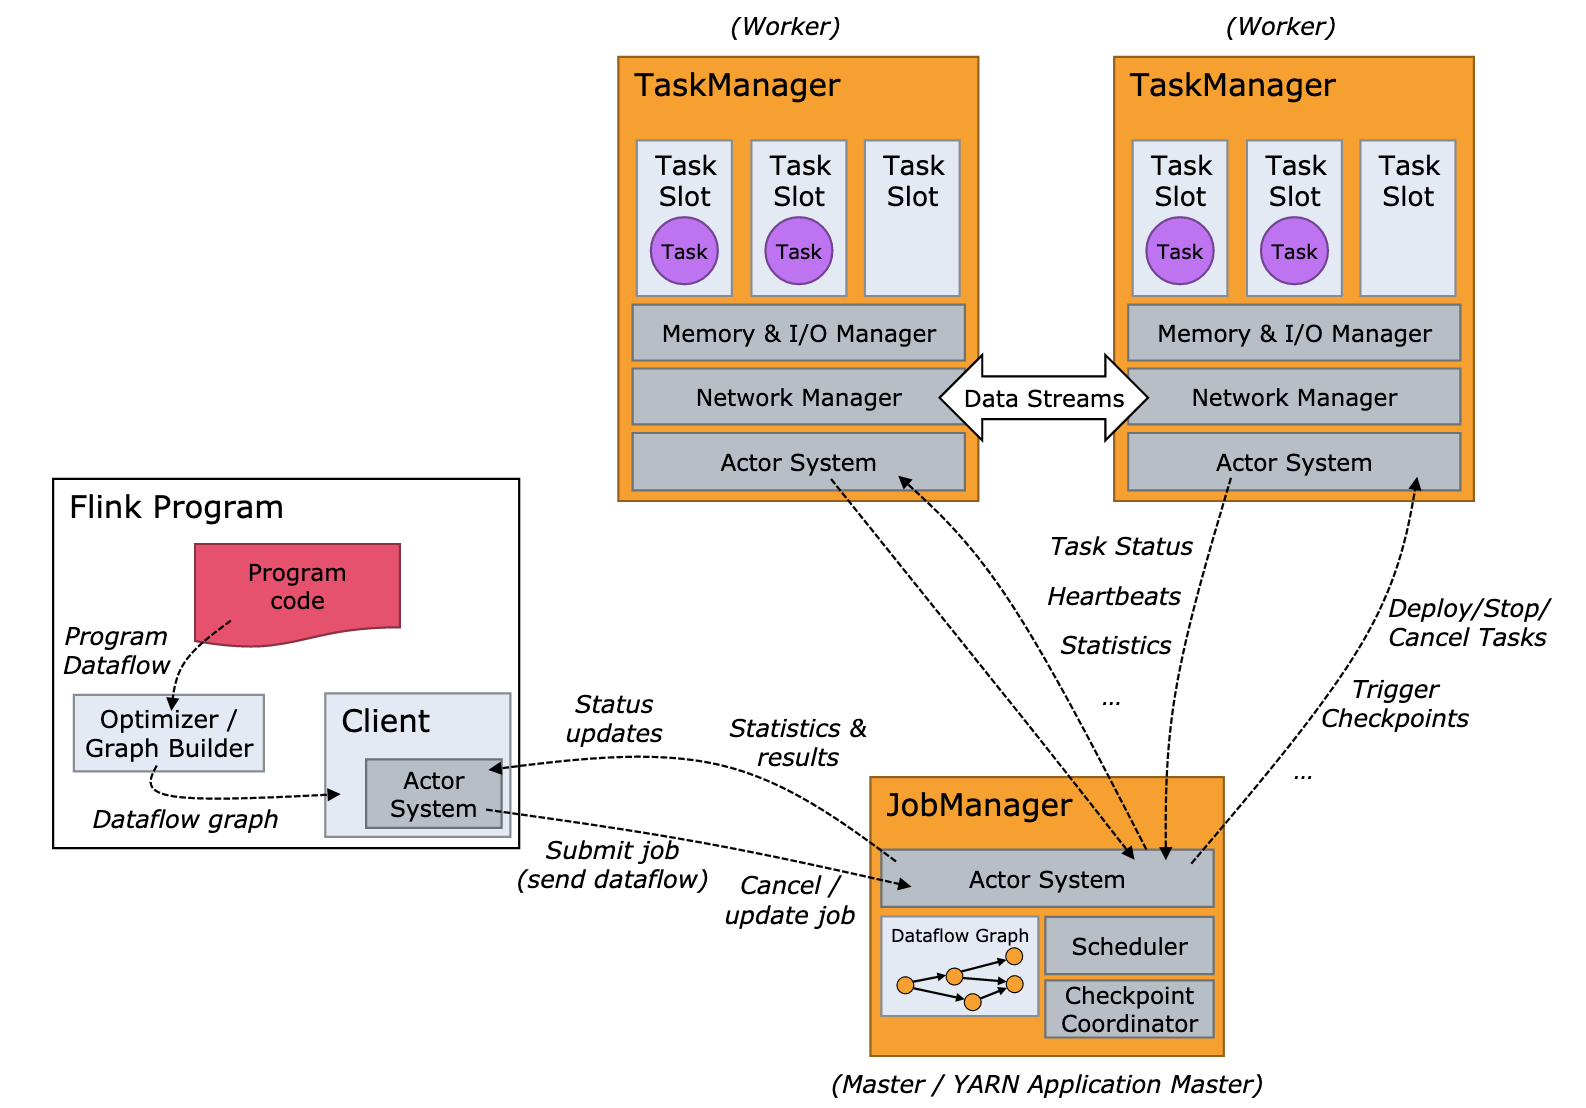
\includegraphics[width=0.8\textwidth]{figuras/processo-flink.png}
% \caption{Processo do \emph{Apache Flink} \cite{ApacheFlink2020}}
% \label{fig:processo-flink}
% \end{figure}

A pilha de componentes de software do \emph{Apache Flink} é composta em camadas.
% da Figura \ref{fig:software-flink}.
A camada \emph{core} é vista como um mecanismo de processamento e execução de
fluxo de dados, enxergando o processamento em lote como um caso especial
\cite{Lopez2018,Carbone2015}.
A camada de APIs é composta pelo \emph{DataStream API}, que processa dados
infinitos ou fluxos de dados, e pelo \emph{DataSet API}, que processa dados
finitos ou dados em lote.
Junto ao \emph{core}, essas APIs montam planos de execução otimizados para cada
tipo de conjuntos de dados, gerando programas executáveis pelo \emph{core}.
Na camada de bibliotecas (\emph{libraries}), há bibliotecas específicas para
cada domínio que geram programas API \emph{Data Stream API} ou \emph{DataSet
API}.
Essas bibliotecas são: \emph{FlinkML} para aprendizado de máquina, \emph{Gelly}
para processamento de grafos, \emph{Table} para domínios relacionais (SQL), e
CEP (\emph{Complex Event Processing}) para processamento de eventos.

\notake{em portugês}
% \begin{figure}[ht]
% \centering
% 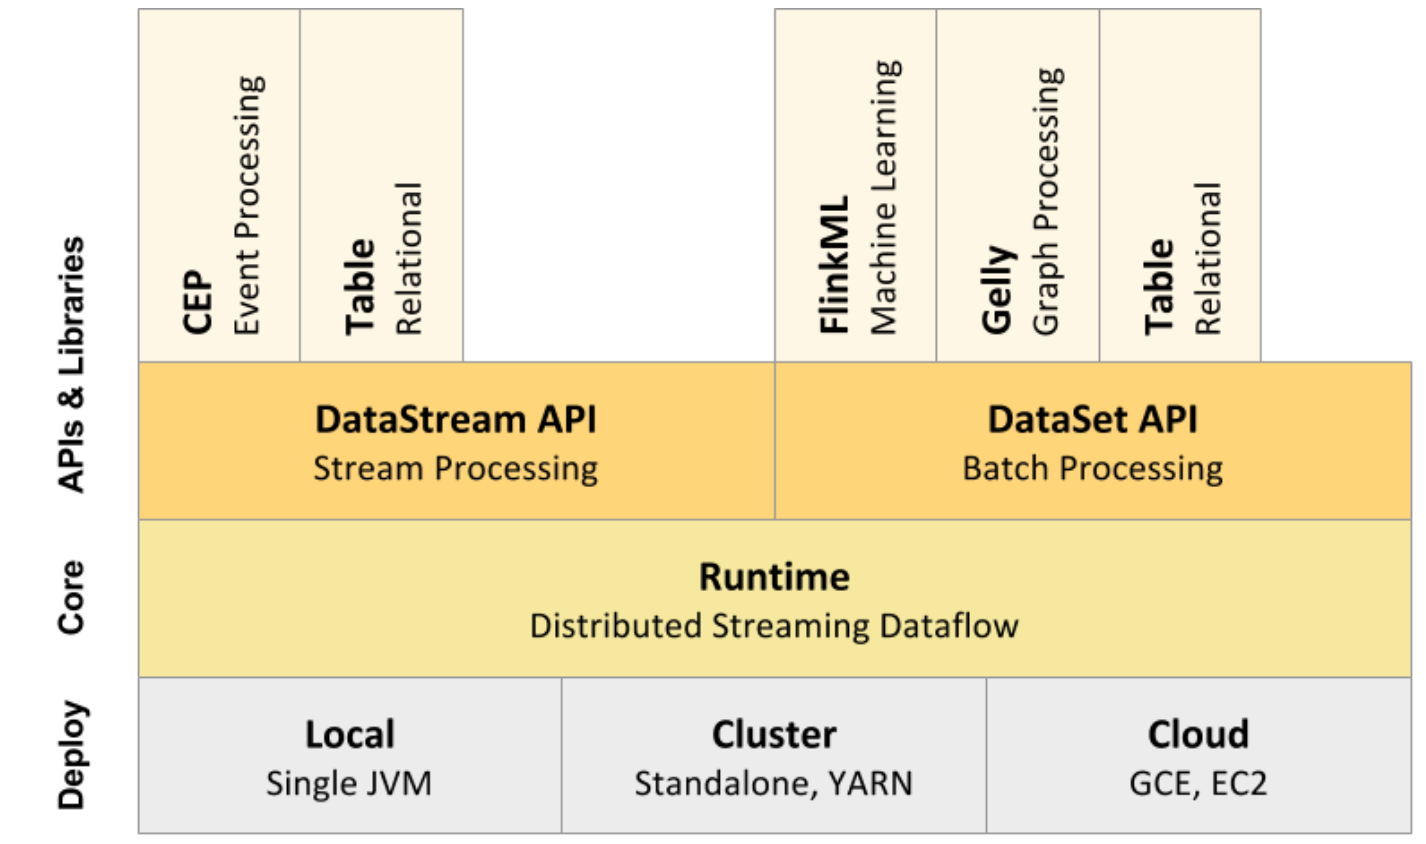
\includegraphics[width=0.7\textwidth]{figuras/software-flink.png}
% \caption{Componentes de software do \emph{Apache Flink} \cite{Carbone2015}.}
% \label{fig:software-flink}
% \end{figure}

\subsection{\emph{Data flow} e \emph{data streams}}

\notafa{aqui eu baguncei os conceitos. Esse data streams é um terminologia do
Apache Flink ou é o data stream que você definiu anteriormente?}
\hlfa{Os \emph{data streams},} ou fluxo de dados, e as transformações são as principais
abstrações do \emph{Apache Flink} \cite{Lopez2018,ApacheFlink2020}.
Um fluxo de dados é definido como um fluxo de registros.
Já as transformações são operações (\emph{map, filtering, reduction, join},
etc.) aplicadas de forma incremental nos \emph{data streams}, gerando um novo
fluxo de dados.
Cada uma dessas transformações pode ser paralelizada por um parâmetro de
paralelismo \cite{Lopez2018}.

Um programa \emph{Flink} é mapeado para um grafo acíclico direcionado, \emph{data
flow}, utilizado pelo \emph{Job Manager} \cite{Carbone2015}.
Esse grafo é composto por operadores de transformação e fluxo de dados
\cite{ApacheFlink2020}.
Para facilitar o paralelismo desse grafo de execução, os operadores que agem
sobre os fluxos de dados podem ser divididos em sub-tarefas que são executadas
pelos \emph{slots} dos \emph{Task Manager}, e os fluxos de dados podem ser
particionados entre os operadores consumidores e produtores.

Cada \emph{data flow} dos programas do \emph{Apache Flink} inicia execução com uma fonte
de dados e termina com um \emph{sink} que escreve os dados de saída em algum
sistema de armazenamento suportado, como \emph{Apache Kafka, Amazon Kinesis Streams,
Hadoop Filesystem} e \emph{Apache Cassandra} \cite{ApacheFlink2020}.
% Na Figura \ref{fig:dataflow-flink}, pode-se observar um exemplo de programa
% \emph{Apache Flink} escrito em Java e seu grafo de execução.
% Nesse exemplo, define-se como fonte de dados o \emph{Apache Kafka}.
% Em seguida, aplica-se uma transformação \emph{map}, e depois outra transformação
% de agrupamento por um dos atributos dos dados e por uma janela de 10 segundos.
% Por fim, o resultado é passado para um \emph{sink}.

% \begin{figure}[ht]
% \centering
% 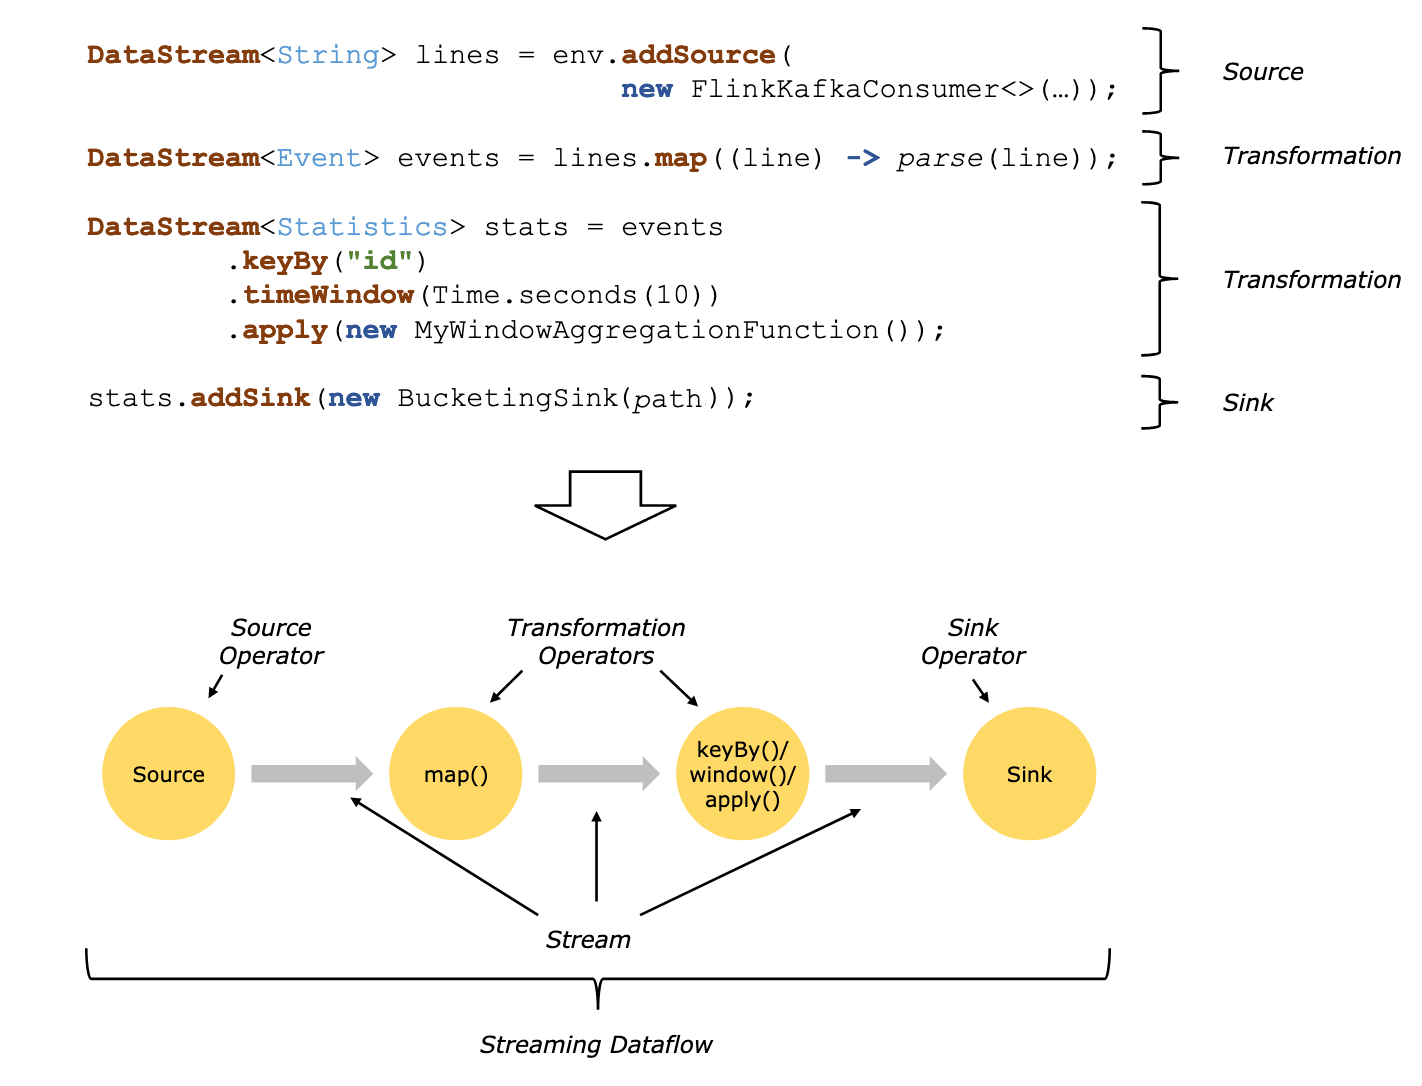
\includegraphics[width=0.85\textwidth]{figuras/dataflow-code-flink.png}
% \caption{Exemplo de código e \emph{data flow} do \emph{Apache Flink} \cite{ApacheFlink2020}}
% \label{fig:dataflow-flink}
% \end{figure}

\subsection{Tolerância a falhas}

O \emph{Apache Flink} implementa um mecanismo de tolerância a falhas combinando repetição e
\emph{checkpoint} dos fluxos \cite{Carbone2015,ApacheFlink2020}.
Um \emph{checkpoint} está relacionado com pontos específicos dos fluxos de
entrada, juntamente com o estado dos operadores.
Um fluxo de dados pode ser retornado a partir de um \emph{checkpoint}, mantendo
a consistência de ``exatamente uma vez'' (não há dados duplicados e nem dados que
não sejam processados), e restaurando o estado dos operadores e eventos naquele
momento.
Portanto, as falhas são tratadas de forma transparente e não afetam a exatidão
da execução de um programa \emph{Flink} \cite{ApacheFlink2020}.

O algoritmo de \emph{checkpoint} assíncrono e incremental \notahl{?}\hlhl{garante} um impacto
mínimo em latência no processamento \cite{Carbone2015}.
Além disso, para reduzir o tempo de recuperação, o \emph{Apache Flink} gera
\emph{snapshots} do estado dos operadores, incluindo a posição atual dos fluxos
de entrada, em intervalos regulares.

% \subsection{Operações com Estado}

O \emph{Apache Flink} realiza computações com estado (\emph{stateful}) que guardam
eventos ou resultados intermediários para acessá-los posteriormente,
contribuindo para planos de execução, mecanismo de recuperação de falhas e para
lembrar de eventos passados para agregar dados \cite{ApacheFlink2020, Carbone2015}.

% \subsection{Processamento em lotes}

O \emph{Apache Flink} considera o processamento em lotes como um caso especial
de fluxo de dados, que nesse caso é limitado em número de elementos.
Para esse tipo de dados existem estruturas de dados e algoritmos específicos, como o
\emph{DataSet API} e operações próprias (agregações, uniões, interações)
\cite{Carbone2015}.

Para o processamento em lote, não há o mecanismo de \emph{checkpoint} como há
para o fluxo de dados.
No lugar, a recuperação é feita repetindo completamente o fluxo ou repetindo as
últimas partições perdidas do fluxo intermediário materializado.

\section{Detecção de Novidade}\label{sec:nd}

\newcommand{\novelty}{\emph{Novelty Detection}\xspace}
\newcommand{\drift}{\emph{Concept Drift}\xspace}
\newcommand{\evolution}{\emph{Concept Evolution}\xspace}

\notafa{(senteça marcada) Alguns autores consideram novidade e anomalia como a
mesma coisa. Outros não (eu sou um dos que não considera)}
\hlfa{No âmbito de classificação de dados,} parte da área de aprendizado de máquina, os
métodos de detecção de novidade (também nomeado detecção de anomalia, \novelty,
\nd) lidam com o reconhecimento e a classificação \hlke{de exemplos que diferem de
exemplos anteriores} \cite{PERNER2007,Gama2010}.
Esses métodos tratam da classificação em fluxos de dados que evoluem com o
tempo, levando em consideração as características desse tipo de fluxos.

% \nota{"As características desse tipo de fluxo de dados são?".. mas que tipo?}

Tratando-se de fluxos de dados contínuos, são características
\notahl{quais?}dos \hlhl{padrões observados}:
evolução de conceito (\evolution) em que novos padrões podem surgir;
desaparecimento ou recorrência de conceito, em que padrões podem desaparecer e
também podem reaparecer;
mudança de conceito (\drift, também nomeado deriva ou desvio) onde um padrão
gradualmente se transforma;
presença de ruído e \emph{outliers} \cite{Gama2010}.

% \nota{separar ai - ndpara\\
% padroes novidade? reconhecomemnto de padroes novidade?}

Os métodos de \nd são utilizados no reconhecimento de \notahl{?}\hlhl{diversos padrões novidade}
ou anomalias e são aplicadas a diversos problemas como
detecção de intrusos \cite{Coull2003,Spinosa2008,Viegas2019,Cassales2019a},
detecção de falhas \cite{Zhang2006},
diagnósticos médicos \cite{Perner2009},
detecção de regiões de interesse em imagens \cite{singh2004approach},
detecção de fraudes \cite{wang2003mining,Abdallah201690}, 
filtros de spam \cite{Hayat2010dct} e
detecção de variações comportamentais em um jogador \cite{Vallim20136258}.

% breve descrição do que sao algoritmos para DN

Alguns métodos tratam de novidades e anomalias como uma classificação de uma
ou duas classes (binariamente) onde um conceito representa a classe normal e
as 
\notafa{frase estranha}
\hlfa{anomalias são representadas pela falta de conceito no modelo} ou
como um segundo conceito no modelo.
No entanto, a abordagem de classificação binária não é adequada para representar
\notafa{alguns trabalhos fazem isso, mas nem todos. É importante destacar que
isso é a visão de um grupo de autor.}
\hlfa{múltiplos conceitos}
em um mesmo conjunto de dados, para isso é necessário abordar
\nd como classificação multi-classe.
Alguns métodos que abordam \nd como classificação multi-classe não
atendem completamente características de conjuntos com 
\notafa{o que é evolução temporal?}
\hlfa{evolução temporal,}
como \evolution e \drift, deixando de detectar múltiplos padrões que surgem
simultaneamente num intervalo de avaliação \cite{Faria2016nd,Gama2010}.

A maioria dos métodos de \nd são construídos seguindo a abordagem de aprendizado
\emph{Offline-Online}. Essa abordagem estabelece que o método seja dividido em
duas fases:
a primeira fase (\emph{Offline}) usa um conjunto de exemplos rotulados para
deles extrair conceitos conhecidos e gerar um modelo;
a segunda fase (\emph{Online}) consome um conjunto ou fluxo de exemplos não
\notafa{um grupo de algoritmos fazem isso, mas nem todos}
\hlfa{rotulados e classifica cada exemplo} em um dos conceitos do modelo, ou marca o
exemplo como desconhecido.
Ainda na segunda fase, para atualizar o modelo, os exemplos marcados como
desconhecidos são utilizados para a extração de novos conceitos ou variações em
conceitos conhecidos \cite{Gama2010}.

Dentre os métodos de \nd que baseiam-se em aprendizado \emph{Offline-Online},
muitos são baseados em algoritmos de agrupamento não supervisionados, tanto
para construção do modelo inicial como na extração de novos conceitos dos
exemplos não explicados pelo modelo marcados como desconhecidos
\cite{Spinosa2009ollinda,Masud2010ECSMiner,Faria2013}.

% Essa abordagem se deve as características 

% \cite{Gama2007,Gama2010,Masud2010ECSMiner,Faria2013,Lavin2015,Abdallah2016anynovel}.

% \cite{Costa2019thesis}

%     - técnicas de Detecção de novidades
% ver se tem algum survey e citar
% (PERNER, 2007)(GAMA, 2010)
% ECSMiner (MASUD et al., 2011)

\section{O algoritmo MINAS}\label{sec:minas-og}

Um algoritmo de \nd que tem recebido atenção nos últimos anos é o algoritmo
MINAS, originalmente proposto por \citeonline{Faria2013}, refinado por
\citeonline{Faria2016minas} e recentemente aprimorado por
\citeonline{DaSilva2018thesis}, com o uso de conceitos \emph{Fuzzy}, e expandido por
\citeonline{Costa2019thesis}, para tratar problemas multi-rótulo além dos problemas
multi-classe já tratados na versão original.
Esse algoritmo segue a abordagem de duas fases no modelo \emph{Offline-Online} e
usa por base algoritmos de agrupamento não supervisionados como \emph{K-means} e
\emph{CluStream}.
% As duas fases, com exceção do método de detecção de padrões novidade da fase
% \emph{Online}, são ilustradas na \reffig{minas}.

% \begin{figure}[ht]
% \centering
% 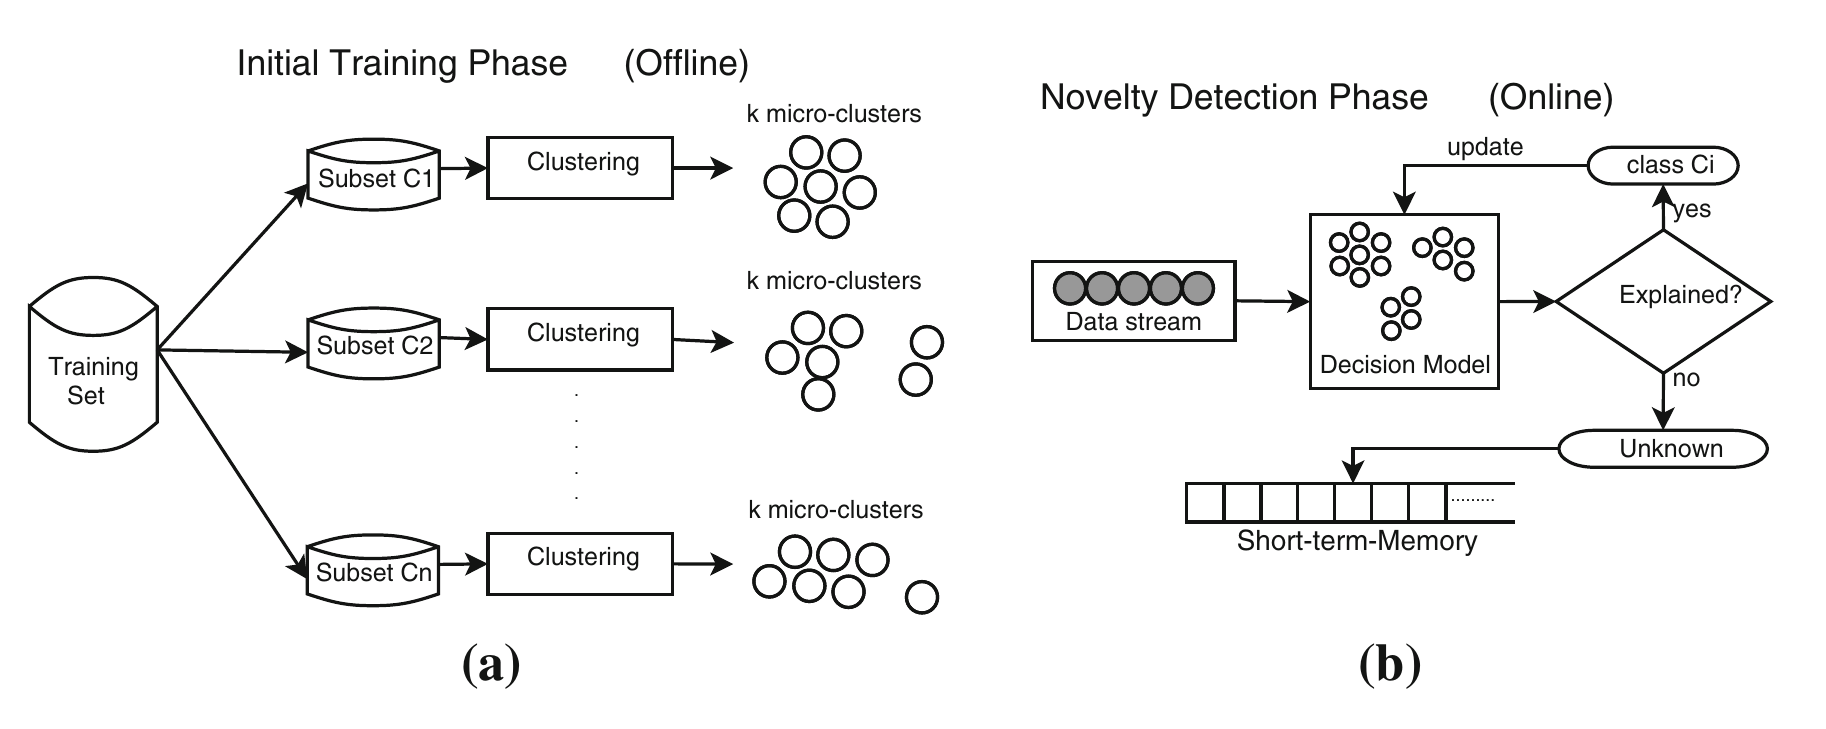
\includegraphics[width=1\textwidth]{figuras/FariaMinas2015-fases.png}
% \caption{Visão geral do algoritmo MINAS com fases \emph{Offline} (a) e 
% \emph{Online} (b) \cite{Faria2016minas}}
% \label{fig:minas}
% \end{figure}

\newcommand{\mcluster}{\emph{micro-cluster}\xspace}
\newcommand{\mclusters}{\emph{micro-clusters}\xspace}

% \nota{talvez mencionar que o minas trabalha no dominio de Double[]}

O algoritmo MINAS em sua fase \emph{Offline} consome um conjunto de treinamento
contendo exemplos etiquetados.
Esse conjunto de treinamento é dividido em grupos usando como chave a etiqueta,
e para cada grupo de exemplos o método de agrupamento (\emph{clustering}) é executado.
O método de agrupamento objetiva resumir um conjunto maior de exemplos em
um conjunto menor de \mclusters que representem por meio de um 
\notafa{essas estatisitcas podem ser deduzidas pelos sumario, mas nao sao o sumario}
\hlfa{sumário,}
contendo, entre outras estatísticas, o centro e raio.
A cada \mcluster é adicionada a etiqueta do grupo original e 
\notahl{?}
\hlhl{todos os conjuntos são unidos} formando o modelo de decisão.

Na fase \emph{Online}, listada no Algoritmo \ref{alg:MINAS}, o algoritmo MINAS
opera com 
\notafa{é composto de duas etapas ou de dois métodos}
\hlfa{dois métodos}.
O primeiro método é o de classificação, onde exemplos do fluxo de dados
são consumidos e avaliados pelo modelo de decisão.
O modelo de decisão avalia cada exemplo calculando a distância euclidiana
entre o exemplo e todos \mclusters do modelo, selecionando o
\mcluster de menor distância.
Se a distância entre o exemplo e o centro do \mcluster for menor que
o raio do \mcluster, o exemplo é classificado com a etiqueta do \mcluster
e o sumário estatístico do \mcluster é atualizado.
Caso a distância (mínima no modelo) seja maior que o raio,
o exemplo é marcado como desconhecido e armazenado
em conjunto próprio.

O segundo método da fase \emph{Online} é a detecção de padrões novidade,
que é executada quando o tamanho do conjunto de desconhecidos é maior
que um parâmetro predefinido.
Esse método executa o agrupamento (\emph{clustering} descrito na fase
\emph{Offline}) e valida os \mclusters gerados verificando sua representatividade
e coesão.

\begin{algorithm}[ht]
  \caption{MINAS \cite{Faria2016minas,Cassales2019a}}
  \label{alg:MINAS}
  \renewcommand{\algorithmicrequire}{\textbf{Entrada:}}
  \begin{algorithmic}[1]
    %T = limiar de distância para pertencer ao grupo
    %P = tempo de "inatividade" para passar para memória sleep
    %ts = limiar para remoção de exemplos da memória temporária
    \REQUIRE $Modelo,FCD,T,NumMinExemplos,ts,P$
    \STATE $MemTmp \leftarrow \emptyset$
    \STATE $MemSleep \leftarrow \emptyset$
    \FORALL{$exemplo \in FCD$}
    \STATE $(Dist,micro) \leftarrow$ micro-mais-proximo($exemplo,Modelo$)
    \IF{$Dist < $ raio($micro$)}
    \STATE $exemplo.classe \leftarrow micro.rotulo$
    \STATE atualizar-micro($micro,exemplo$)
    \ELSE
    \STATE $exemplo.classe \leftarrow desconhecido$
    \STATE $MemTmp \leftarrow MemTmp \cup exemplo$
    \IF{$|MemTmp| \geq NumMinExemplos$}
    \STATE $Modelo \leftarrow $ deteccao-novidade($Modelo,MemTmp,T$)
    \ENDIF
    \ENDIF
    \STATE $TempoAtual \leftarrow exemplo.T$
    \IF{$TempoAtual$ mod $TamJanela == 0$}
    \STATE $Modelo \leftarrow$ mover-micro-grupos-mem-sleep($Modelo,MemSleep,P$)
    \STATE $MemTmp \leftarrow$ remover-exemplos-antigos($MemTmp,ts$)
    \ENDIF
    \ENDFOR
  \end{algorithmic}
\end{algorithm}

Para atribuição de etiquetas aos \mclusters gerados, o algoritmo MINAS
encontra no modelo atual o \mcluster mais próximo pela distância
euclidiana e classifica em dois tipos de conceito.
Se a distância é menor que um parâmetro predefinido,
o novo \mcluster gerado recebe como etiqueta o valor de extensão
de conceito conhecido.
Caso contrário, se o novo \mcluster está mais distante,
um novo conceito foi encontrado e a etiqueta marca um padrão novidade.
Após a atribuição da etiqueta do novo \mcluster, ele é adicionado
ao modelo de decisão.

% Although efficient in detecting NP, MINAS is
% very sensitive to noisy data and data scale, what causes a
% decrease in its accuracy. \cite{DaSilva2018}

% ver paper da profa. Elaine

% % discussão de 2020-02-01
% Detecção de intrusão em redes
%     - riscos de segurança
%     % pontos de coleta de dados básicos para a maioria das estruturas de IoT sao Wireless Sensor Networks (WSN) e WSN baseadas em IP,
%     % as quais s˜ao vulneráveis e geram uma ameac¸a de seguranc¸a de alto n´ıvel (ADAT; GUPTA, 2018) Adat2018
%     % (KASINATHAN et al., 2013), a detecc¸ ˜ao de assinaturas
%     % (RAZA; WALLGREN; VOIGT, 2013; SHEIKHAN; BOSTANI, 2016) s˜ao propostos IDSs h´ıbridos com foco 
%                 % espec´ıfico em ataques de roteamento como sink-hole e redireciona- mento seletivo
%     - técnicas de intrusão e tipos de ataques
%     - mecanismo de detecção (análise de fluxo de rede -> detecção de anomalia)
%     % Guilherme: A tarefa de detecção de intrusão consiste em descobrir, 
%     %           determinar e identificar a utilização, duplicação, alteração ou destruição
%     %           não autorizada de sistemas de informação (MUKKAMALA; SUNG; ABRAHAM, 2005) Mukkamala2005
%     % deteccao por assinaturas (tambem chamada de misuse-detection), deteccao comportamental (tambem chamada de anomaly-detection)e deteccao hıbrida.(MODI et al., 2013).
%     % implementacao usualmente é feita por meio de técnicas de AM e MD (BUCZAK; GUVEN, 2016).
%     % existem poucos trabalhos [..] online e deteccao de novidade ao problema [..] observado nas surveys (BUCZAK; GUVEN, 2016; MITCHELL; CHEN, 2014; MODI et al., 2013).
%     % (FURQUIM et al., 2018), os autores implementam uma arquitetura de 3 camadas (WSN, Fog e Cloud)
%     % (MIDI et al., 2017), os autores propuseram um IDS h´ıbrido [...] ativa apenas os módulos [...] especializado em um ataque espec´ıfic
%     % (FAISAL et al., 2015)externo ou interno ao Smart Meter.dados do KDD99 [...] precis˜ao, Kappa, consumo de memória, tempo e FAR
%     % extensivamente em (Sommer; Paxson, 2010) e (MCHUGH, 2000), é dif´ıcil encontrar boas me- didas de avaliac¸ ˜ao para IDSs
%     % (GAMA, 2010) afirma que no contexto de processamento de fluxo, as medidas tradicionais s˜ao impreci- sas.
% Detecção de novidades
%     % (PERNER, 2007)(GAMA, 2010). A
%     - técnicas de Detecção de novidades
%     - MINAS (incluir métricas) 
%     % (FARIA et al., 2016)
%     % ECSMiner (MASUD et al., 2011)
%     % AnyNovel (ABDALLAH et al., 2016) s˜ao
%     % medidas de Qualidade da Deteccao utilizadas foram Fnew, Mnew, Erro e a quantidade de exemplos rotulados por especialistas que cada técnica requisitou (MASUD et al., 2011)
%     - BigFlow (incluir métricas)
% Processamento de Streams (big data)
%     - cloud?
%     % A arquitetura Lambda (MARZ; WARREN, 2015) de duas camadas de CPU (stream e batch) e camada de serviço
%     % Kappa (KREPS, 2014) possui apenas um módulo de processamento on-line (apenas as camadas de processamento e servic¸o)
%     - redes como stream
%     - Atraso
%     - Kafka/Spark/Flink
% Redes IoT
%     - Restrição hardware (Energia, CPU, Mem, Rede)
%     - Consideração FOG vs Cloud
% %/discussão


% \section{Algoritmos de Detecção de Novidades}\label{sec:alg-nd}

\newcommand{\cluster}{\emph{cluster}\xspace}
\newcommand{\clusters}{\emph{clusters}\xspace}

\newcommand{\dataset}{\emph{data set}\xspace}
\newcommand{\datasets}{\emph{data sets}\xspace}
% \clusters é um conjunto de \cluster feito de um \dataset.

O algoritmo MINAS, como já foi discutido na Seção \ref{sec:minas-og}, classifica
exemplos e detecta
novidades em DS e considera em sua composição \emph{concept drift} e
\emph{concept evolution}, sendo capaz de classificar como extensão de classe
conhecida e identificar padrões novidade sem intervenção de especialista
\cite{Faria2016minas}.
Neste trabalho, consideram-se algoritmos derivados do algoritmo MINAS
aqueles apresentados em trabalhos publicados após 2016, que estendem a
implementação original seguindo sua estrutura básica.

\subsection{Algoritmo FuzzyND}

% FuzzyND
% $(n, \mathit{M}, \overline{CF1^x}, SSD^e, t, l)$
% $(n, LS, SS, t, l)$
% A nova estrutura contrapõem a estrutura original
% substituindo a soma linear dos elementos ($LS$) por  e $SS$ por $M$ e $$

O algoritmo FuzzyND, derivado do MINAS foi proposto por \citeonline{DaSilva2018}.
FuzzyND incrementa o algoritmo original, aplicando a ele teorias de
conjuntos \emph{fuzzy} pela modificação da representação dos \clusters.
A modificação afeta o método de construção de \clusters, método de classificação
de exemplos e método de detecção de novidades de acordo com a nova representação.

\acronym{F1M}{\emph{Macro F-Score}, acurácia }

A avaliação do algoritmo FuzzyND foi feita por meio de experimentos usando 3 
\datasets sintéticos (\emph{MOA3}, \emph{RBF}, \emph{SynEDC})
e por comparação com o MINAS.
O método de avaliação utilizado baseia-se na matriz de confusão incremental
descrita por \citeonline{Faria2016nd}, extraindo dessa matriz duas métricas:
acurácia (\emph{Macro F-Score}) \cite{Sokolova2009} e
taxa de desconhecidos (\emph{UnkR}) \cite{Faria2016minas}.
Em geral, o algoritmo FuzzyND detecta melhor novidades e, consequentemente,
é mais robusto a valores atípicos (\emph{outlier}), porém perde a capacidade
de reconhecer padrões recorrentes.


% Experiments were evaluated using the incremental confusion-matrix proposed by [27],
% recently been proposed [5]–[9]
% [5] T. Al-Khateeb, M. M. Masud, L. Khan, C. Aggarwal, J. Han, and B.
% Thuraisingham, “Stream classification with recurring and novel class detection
% using class-based ensemble,” in Data Mining (ICDM), 2012 IEEE 12th International
% Conference on. IEEE, 2012, pp. 31–40.
% [6] E. R. de Faria, A. C. P. de Leon Ferreira, J. Gama et al., “Minas:
% multiclass learning algorithm for novelty detection in data streams,” Data
% Mining and Knowledge Discovery, vol. 30, no. 3, pp. 640–680, 2016.
% [7] M. Masud, J. Gao, L. Khan, J. Han, and B. M. Thuraisingham, “Classification
% and novel class detection in concept-drifting data streams under time
% constraints,” IEEE Transactions on Knowledge and Data Engineering, vol. 23, no.
% 6, pp. 859–874, 2011.
% [8] M. M. Masud, Q. Chen, L. Khan, C. Aggarwal, J. Gao, J. Han, and B.
% Thuraisingham, “Addressing concept-evolution in concept-drifting data streams,”
% in Data Mining (ICDM), 2010 IEEE 10th International Conference on. IEEE, 2010,
% pp. 929–934.
% [9] Z. S. Abdallah, M. M. Gaber, B. Srinivasan, and S. Krishnaswamy, “Anynovel:
% detection of novel concepts in evolving data streams,” Evolving Systems, vol. 7,
% no. 2, pp. 73–93, 2016.
% [27] E. R. de Faria, I. R. Goncalves, J. Gama, A. C. P. de Leon Ferreira et al.,
% “Evaluation of multiclass novelty detection algorithms for data streams,” IEEE
% Transactions on Knowledge and Data Engineering, vol. 27, no. 11, pp. 2961–2973,
% 2015.
% [28] M. Sokolova and G. Lapalme, “A systematic analysis of performance measures
% for classification tasks,” Information Processing & Manage- ment, vol. 45, no.
% 4, pp. 427–437, 2009.

\subsection{Algoritmos MINAS-LC e MINAS-BR}\label{sub:minas-derivados}

O algoritmo MINAS-LC foi proposto por \citeonline{Costa2019thesis} e trata a classificação
multi-rótulo, porém não trata evoluções de conceito (\emph{Concept Evolution}).
As alterações fundamentais propostas são:
a representação de \cluster onde MINAS-LC troca a etiqueta, que era única, por uma multi-rótulo;
a transformação de problema aplicada ao conjunto de treinamento para transformá-lo de um
conjunto multi-rótulo para um conjunto multi-classe (simplificação)
em duas variações \emph{Label Powerset} e \emph{Pruned Sets} com
mineração de conjunto de itens frequentes.

% Este capítulo apresentou o método MultI-label learNing Algorithm for data
% Streams with Label Combination-based methods (MINAS-LC) e o MultI-label learNing
% Algorithm for data Streams with Binary Relevance transformation (MINAS-BR) para
% CMFCD com latência extrema de rótulos. O MINAS-LC lida com problemas apenas com
% mudanças de conceito. O seu modelo de decisão e composto por microgrupos
% multirrotulados sendo capaz de classificar exemplos em várias classes
% simultaneamente e evoluir ao longo do fluxo de dados. Foram propostas duas
% variações do método: utilizando o método de transformação de problema Label
% Powerset (LP) e, utilizando o método Pruned Sets (PS) com mineração de conjunto
% de itens frequentes. O MINAS-BR lida com problemas tanto com mudanças de
% conceito, como com evo- luções de conceito. Ele possui um conjunto de modelos de
% decisão, um para cada classe do problema. Esses modelos de decisão podem ser
% entendidos adaptando-se às mudanças de con- ceito, ou novos modelos de decisão
% podem ser criados, adaptando-se às evoluções de conceito. O próximo capítulo
% apresenta os experimentos realizados envolvendo os dois métodos propostos neste
% trabalho.

Já o trabalho de \citeonline{Costa2019}, estende o algoritmo original para que
classifique um exemplo com uma ou mais etiquetas usando a transformação
\emph{Binary Relevance}, o que deu origem ao algoritmo MINAS-BR.
O algoritmo modifica a representação do modelo, originalmente conjunto de \clusters, para
um grupo de \clusters por classe (etiqueta).
Também modifica o método de agrupamento, substituindo a inicialização do 
algoritmo \emph{K-means}, originalmente aleatória, pelo algoritmo 
\emph{Leader Incremental Clustering} \cite{Vijaya2004505}.

% as 4CRE-V13, 4CRE-V24 e 5CVT5 6 foram geradas originalmente em Souza et al. (2015b)
% SOUZA, V. M. A.; SILVA, D. F.; GAMA, J.; BATISTA, G. E. A. P. A. Data stream
% classification guided by clustering on nonstationary environments and extreme
% verification latency. In: Procee- dings ofSIAM International Conference on Data
% Mining (SDM). [S.l.: s.n.], 2015. p. 873–881. Citado 4 vezes nas páginas 17, 65,
% 87 e 89.

O algoritmo MINAS-BR também é experimentalmente avaliado com 4 \emph{data sets}
sintéticos: \emph{MOA-3C-5C-2D}, \emph{MOA-5C-7C-2D}, \emph{MOA-5C-7C-3} da
ferramenta MOA \cite{MOA} e \emph{4CRE-V2}
\footnote{
    A versão original do \dataset 4CRE-V2 está disponível em 
    https://sites.google.com/site/nonstationaryarchive/home
}
gerados pelo método \emph{Radial Basis Function} \cite{souza2015}.
O algoritmo MINAS-BR foi comparado com 7 algoritmos da literatura também disponíveis na ferramenta
MOA \cite{MOA},
diferente da avaliação do FuzzyND que compara diretamente com MINAS.
Para análise, os 7 algoritmos foram divididos em dois grupos.
O primeiro grupo de 3 algoritmos com acesso às etiquetas corretas para
atualização do modelo e com a técnica ADWIN (\emph{ADaptive WINdowing}) para detectar
mudanças de conceito (\emph{Concept Drift})
O segundo grupo com os 4 algoritmos sem acesso às etiquetas corretas,
ou seja, sem \emph{feedback} externo, mesma condição do MINAS-BR.

% Esse trecho parece mais fundamentação.

A avaliação elencada por \citeonline{Costa2019} leva em consideração que as classes
contidas no conjunto de testes podem não ter correlação direta com os padrões identificados
pelos algoritmos.
Para tratar a divergência, uma estratégia baseada em proposta anterior por
\citeonline{Faria2016nd} foi apresentada com alterações para exemplos multi-rótulo.
Após associação entre padrões de novidade e classes novidade foi possível calcular
métricas tradicionais.
A estratégia é executada na fase de classificação seguindo as regras:

\begin{enumerate}

    \item após o consumo do exemplo $X_n$;
    
    \item para todo padrão $P_i$ (etiqueta atribuída) identificado sem
    associação até o momento;
    
    \item com classes novidade $y_j$ (etiqueta real) presentes em exemplos antes
    $X_n$;
    
    \item preenche-se a tabela de contingência $\mathbf{T}_{(i,j)}$ relacionando
    padrão $P_i$ e classe $y_j$;
    
    \item calcula-se o grau de dependência $\mathit{F1}$ derivado da tabela de
    contingência $\mathit{F1}_{(i,j)} = f(\mathbf{T}_{(i,j)})$;
    
    \item valores $\mathit{F1}_{(i,j)} = 0$ são descartados;
    
    \item dentre os valores restantes: o padrão $P_i$ é associado à classe $y_j$
    se $\mathit{F1}_{(i,j)}$ é máximo.

\end{enumerate}

As métricas utilizadas por \citeonline{Costa2019} após a associação de classes e
padrões são as tradicionais taxa de desconhecidos (\emph{UnkRM}) e \emph{F1M}.
Os resultados apresentados indicam que MINAS-BR capturou todas as novidades dos
\datasets sintéticos de teste e mostrou, como esperado, melhores métricas que os
4 algoritmos equivalentes da literatura ficando abaixo dos 3 com \emph{feedback}
externo.

Os trabalhos relacionados nessa \refsec{alg-nd}, têm em
comum, além do algoritmo base, as métricas de avaliação acurácia (\emph{Macro F-Score} e \emph{Macro
F-Measure} F1M) e taxa de desconhecidos, aplicadas com devido tratamento.
Também é comum entre eles o uso de \datasets sintéticos.
Outro potencial não explorado do MINAS é em aplicações reais, ou seja,
consumindo além de \datasets reais, fluxos realistas em ambientes simulados ou
reais porém considerando uso de recursos computacionais.

Observando a arquitetura dos algoritmos abordados na \refsec{alg-nd}, nota-se as semelhanças:
a fase offline centrada no processo de agrupamento e criação de modelo;
a fase online dividida em classificação (com atualização das estatísticas do modelo)
e detecção de padrões, onde novamente o processo de agrupamento é central.
Portanto, apesar de outros trabalhos expandirem o algoritmo com diferentes técnicas, seu
núcleo continua relevante\footnote{
Propostas de modificação do algoritmo MINAS estão longe de serem exauridas.
Não cabe ao presente trabalho expandir e validar conceitos de aprendizagem de máquina,
porém alguns exemplos mencionados ainda não abordados são:
\begin{enumerate*}[label={\alph*)}]
    
    \item diferentes métodos de cálculo de distância entre pontos além da
    distância euclidiana;
    
    \item a mudança de representação de \clusters, atualmente hiper-esferas
    \cite{Costa2019thesis}, para hiper-cubos tratando \datasets onde as
    características representadas pelas dimensões são completamente
    independentes;
    
    \item um modo interativo onde o \cluster é formado, mostrado ao especialista
    que o classifica como inválido (ruído ou não representativo) ou válido,
    podendo conter uma ou mais classes e, se contiver mais que uma classe corte em
    grupos menores até conter somente uma classe;
    
    \item ainda considerando interação com especialista, a possibilidade de
    injetar um exemplo não pertencente a uma classe, ou seja, marcar o exemplo
    como não pertencente a uma classe para mantê-lo na memória de
    desconhecidos e, eventualmente forçar criação de um \cluster que represente
    uma classe geometricamente próxima mas semanticamente distinta;
    
    \item na fase \emph{offline} a verificação de sobreposição de \clusters
    pertencentes a classes distintas e tratamento adequado.

\end{enumerate*}
} \cite{DaSilva2018,DaSilva2018thesis,Costa2019}.

% >>>>>>> master
% \citeonline{DaSilva2018}

% \citeonline{Costa2019} estende o algoritmo original na sua capacidade de
% classificar um exemplo com uma ou mais etiquetas usando a transformação
% \emph{Binary Relevance}. Essa versão modificada é testada e comparada com 7
% algoritmos por meio de experimentos com 4 \emph{data sets} sintéticos gerados
% pelo método \emph{Radial Basis Function}. Os 7 algoritmos e o método estão
% disponíveis na ferramenta MOA \cite{MOA}.
% w

% Apesar de outros trabalhos expandirem o algoritmo com diferentes técnicas, seu
% núcleo continua relevante \cite{DaSilva2018,DaSilva2018thesis,Costa2019}.
% <<<<<<

% \section{AnyNovel}
% \nota{Incompleto}

% \nota{também é da mesma classe do minas porém \citeonline{Cassales2019a} destaca um
% desempenho inferior para o \emph{data set} testado.}
%  a atividade de detecção de intrusão

% \citeonline{Abdallah2016anynovel}

% \nota{helio: Mining wireless networks}